% Options for packages loaded elsewhere
\PassOptionsToPackage{unicode}{hyperref}
\PassOptionsToPackage{hyphens}{url}
%
\documentclass[
]{book}
\usepackage{amsmath,amssymb}
\usepackage{lmodern}
\usepackage{iftex}
\ifPDFTeX
  \usepackage[T1]{fontenc}
  \usepackage[utf8]{inputenc}
  \usepackage{textcomp} % provide euro and other symbols
\else % if luatex or xetex
  \usepackage{unicode-math}
  \defaultfontfeatures{Scale=MatchLowercase}
  \defaultfontfeatures[\rmfamily]{Ligatures=TeX,Scale=1}
\fi
% Use upquote if available, for straight quotes in verbatim environments
\IfFileExists{upquote.sty}{\usepackage{upquote}}{}
\IfFileExists{microtype.sty}{% use microtype if available
  \usepackage[]{microtype}
  \UseMicrotypeSet[protrusion]{basicmath} % disable protrusion for tt fonts
}{}
\makeatletter
\@ifundefined{KOMAClassName}{% if non-KOMA class
  \IfFileExists{parskip.sty}{%
    \usepackage{parskip}
  }{% else
    \setlength{\parindent}{0pt}
    \setlength{\parskip}{6pt plus 2pt minus 1pt}}
}{% if KOMA class
  \KOMAoptions{parskip=half}}
\makeatother
\usepackage{xcolor}
\usepackage{longtable,booktabs,array}
\usepackage{calc} % for calculating minipage widths
% Correct order of tables after \paragraph or \subparagraph
\usepackage{etoolbox}
\makeatletter
\patchcmd\longtable{\par}{\if@noskipsec\mbox{}\fi\par}{}{}
\makeatother
% Allow footnotes in longtable head/foot
\IfFileExists{footnotehyper.sty}{\usepackage{footnotehyper}}{\usepackage{footnote}}
\makesavenoteenv{longtable}
\usepackage{graphicx}
\makeatletter
\def\maxwidth{\ifdim\Gin@nat@width>\linewidth\linewidth\else\Gin@nat@width\fi}
\def\maxheight{\ifdim\Gin@nat@height>\textheight\textheight\else\Gin@nat@height\fi}
\makeatother
% Scale images if necessary, so that they will not overflow the page
% margins by default, and it is still possible to overwrite the defaults
% using explicit options in \includegraphics[width, height, ...]{}
\setkeys{Gin}{width=\maxwidth,height=\maxheight,keepaspectratio}
% Set default figure placement to htbp
\makeatletter
\def\fps@figure{htbp}
\makeatother
\setlength{\emergencystretch}{3em} % prevent overfull lines
\providecommand{\tightlist}{%
  \setlength{\itemsep}{0pt}\setlength{\parskip}{0pt}}
\setcounter{secnumdepth}{5}
\usepackage{booktabs}
\ifLuaTeX
  \usepackage{selnolig}  % disable illegal ligatures
\fi
\usepackage[]{natbib}
\bibliographystyle{plainnat}
\IfFileExists{bookmark.sty}{\usepackage{bookmark}}{\usepackage{hyperref}}
\IfFileExists{xurl.sty}{\usepackage{xurl}}{} % add URL line breaks if available
\urlstyle{same} % disable monospaced font for URLs
\hypersetup{
  pdftitle={Project Targeting Index (PTI): Guideline},
  pdfauthor={Takaaki Masaki},
  hidelinks,
  pdfcreator={LaTeX via pandoc}}

\title{Project Targeting Index (PTI): Guideline}
\author{Takaaki Masaki}
\date{2022-09-02}

\begin{document}
\maketitle

{
\setcounter{tocdepth}{1}
\tableofcontents
}
\hypertarget{introduction}{%
\chapter{Introduction}\label{introduction}}

Tracking how the World Bank's portfolio of activities aligns with evolving circumstances in specific countries is challenging. World Bank teams engage with countries through important strategic and prioritization exercises, such as the Country Partnership Framework (CPF) and the Systematic Country Diagnostic (SCD). To maximize the development benefits of activities identified under these activities, it is essential to ensure that projects and programs evolve with changing circumstances while reaching the areas that are most in need.

The PTI offers a framework for project and country teams to match objectives with geographic project site selection. Teams can ensure that project site selection aligns with the country strategy, and the country management unit (CMU) can monitor consistency between project sites and the country strategy. Spatially targeting the Bank's interventions based on objective criteria and evidence also helps inject transparency into project site selection and promote efficiency in reaching intended beneficiaries. Teams can use the PTI online dashboard, which serves both as a database of subnational indicators and as a user-friendly tool for PTI calculation, to track fast-changing emergency situations. In Morocco, for instance, the PTI online tool can map reported COVID-19 cases to a battery of subnational socio-economic indicators.

The purpose of this guideline is to provide a guideline on how to create a PTI dashboard. It breaks down the process of building a PTI dashboard into four different phases as shown in the diagram below. The book consists of four chapters that correspond to these four steps: \protect\hyperlink{identification}{Identification (Chapter 2)}; PTI preparation (Chapter 3); Application (Chapter 4); and Monitoring (Chapter 5).

\begin{figure}
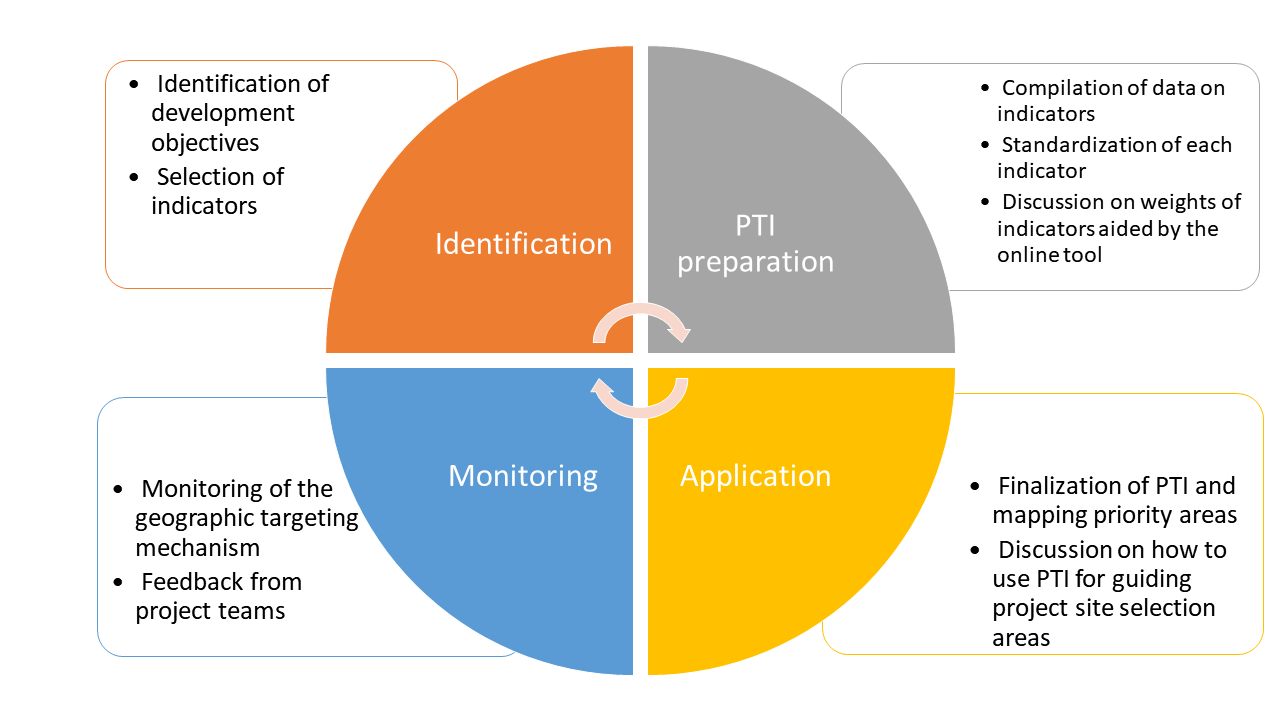
\includegraphics[width=1\linewidth]{figure1/Slide1} \caption{Lifecycle of the PTI project}\label{fig:pressure}
\end{figure}

\hypertarget{identification}{%
\chapter{Identification}\label{identification}}

First, identify development objectives. A clear set of development objectives that can be measured objectively by data and evidence, and established in close coordination with the respective country teams, lays the groundwork for PTI mapping. Goals outlined in a Country Partnership Framework (CPF) are a good starting point to guide selection of development objectives.

\hypertarget{pti-prep}{%
\chapter{PTI preparation}\label{pti-prep}}

Second, identify indicators pertaining to the specific objectives. Once development objectives are agreed upon among stakeholders, indicators pertaining to those specific objectives are identified. Since PTI informs spatial targeting, these indicators need to be available at a subnational level (for example, villages, districts, regions, provinces). People most familiar with the country context---project teams, country experts. and sector specialists---should provide input on indicator selection. Teams may also consult GIS specialists in this selection process as a rich source of high-resolution socio-economic data is now available to inform spatial targeting at a highly disaggregated level.

\hypertarget{application}{%
\chapter{Application}\label{application}}

Third, construct a composite weighted index. Once a set of indicators has been identified, these indicators are aggregated to construct a composite index. Often, some indicators vary significantly across a country. One example is the number of poor people living in each district. If such an indicator is combined with other indicators with limited variation, the composite PTI indicator tends to heavily reflect the geographic pattern of the poor population. To avoid this, the PTI standardizes all indicators to have mean and variance of 0 and 1 respectively. These standardized indicators are then combined into a composite index. The PTI aggregates the standardized indicators with weights, which reflect the relative importance of each variable. As the weight of an indicator increases, the geographic distribution of priority areas of PTI is more affected by that indicator. To facilitate the process of choosing which weights to assign to different indicators, the PTI tool includes an interactive online dashboard that creates a map of priority areas based on selection of indicators and weights so that country team members can easily see the implications that changing weights have on the map of priorities.

\hypertarget{monitoring}{%
\chapter{Monitoring}\label{monitoring}}

Fourth, construct final PTI. Based on the country team consensus on weighted indicators, a final PTI and corresponding map of priority areas is constructed.

  \bibliography{book.bib,packages.bib}

\end{document}
